\chapter{绪论}

\section{课题背景}{
	\begin{figure}[htbp]
	\centering
	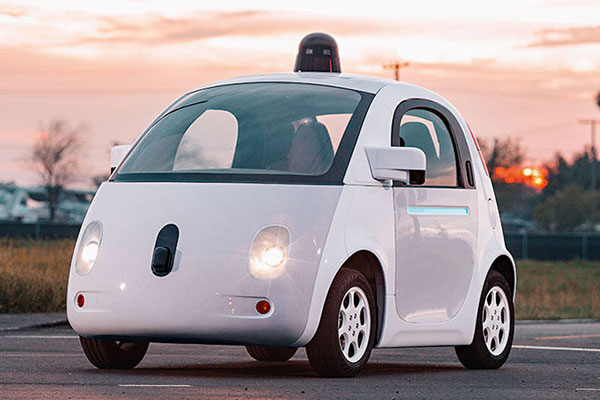
\includegraphics[width=5in]{images/WRC.jpg}
	\caption{Google无人车}
	\label{WRC}
	\end{figure}
	当下机器学习发展迅猛,机器学习渗透进入了许多领域,为很多问题的处理带来了新思路、新方案,是未来计算机领域发展的一个很有前景的趋势。而在机器学习普及的同时,智能驾驶成为一个非常热门的方向。智能驾驶是一个非常复杂的系统,包括对实时数据的收集(如传感器),对当前状况的预测(如行人检测),对之后状态的决策(如轨迹生成),控制车辆操作。近来全球都刮起了一股无人车驾驶的热潮,从最开始的实验室领头,到后来国外的google、特斯拉、Uber,国内的百度、图森、滴滴,智能驾驶成为一个非常火热的方向。不久前刚在美国加州领到无人车驾驶证的百度,又或者曾经在KITTI数据集第一的图森,又或者是已经将无人车商业化的特斯拉都在致力于成为无人驾驶领域的领军企业。而行人检测就是自动驾驶(或辅助驾驶)中相当重要的一环,而保证行人检测的准确性和实时性自然是相当重要的事情,本项目便是基于智能驾驶的背景,探究行人检测的新算法、新模型,实现实时的行人检测。

	行人检测是一种典型的物体检测。行人检测具有极其广泛的应用:智能辅助驾驶,智能监控,行人分析以及智能机器人等领域,在过去几年中引起了广泛的关注。目前传统的行人检测方法大多是使用的滑动窗口,特征提取,然后分类建模,如积分通道特征的方法。对于相关论文的研究\cite{walk2010new,integral},传统行人检测算法能分为两类:
	\begin{enumerate}
	\item 基于背景建模:利用背景建模方法,提取出前景运动的目标,在目标区域内进行特征提取,然后利用分类器进行分类,判断是否包含行人
	\item 基于统计学习:这也是目前行人检测最常用的方法,根据大量的样本构建行人检测分类器。提取的特征主要有目标的灰度、边缘、纹理、颜色、梯度直方图等信息。
	\end{enumerate}

	而实时行人检测也是一个比较复杂的问题。在实验过程中,使用的图片大多都是光照充足,物体特征明确的情况。而在实际的问题中,我们不得不面对光照改变的情况,或者天气变化的情况,甚至行人之间也会有重合的情况。实际的复杂情况大大加大了行人检测预测准确的难度,而车辆驾驶的实时性也对行人检测预测的速度要求更高。

	得益于硬件设备的提升,深度学习在近几年发展迅猛,深度学习通过构建一个深层的网络结构,通过监督学习的方法来构建一个物体检测的模型。而卷积神经网络就是其中很重要的一个分支,卷积神经网络与其他神经网络不同之处在于它通过每一层的卷积核去处理图像信息。由于对局部特征处理效果好,参数少训练快,网络结构复杂可塑性强,卷积神经网络成为处理图像信息的一个主流的方向。在物体检测上,基于卷积神经网络的模型\cite{yolo,faster,ssd,fast,rich}也是层出不穷,效果越来越好,速度越来越快。

	卷积神经网络在目标识别检测上取得了巨大的成功,而目前行人检测领域的主流结果仍采用积分通道特征。本项目将从之前的研究成果出发,参考近来比较火热的物体检测的卷积神经网络,研究面向主动驾驶安全的行人检测算法。本项目将参考YOLO的网络模型,在主流的行人数据集上,对比各模型的准确率和速度,探讨实时行人检测的方案与技术。

	针对上述问题以及技术背景,在导师的指导下,提出了本项目的设计课题:面向实时行人检测的快速卷积神经网络研究。
}

\section{本文研究目标和内容}{
	本项目的全称为面向实时行人检测的快速卷积神经网络研究。该项目是从KITTI的数据集中下载训练和测试的图片和标签,将数据集预处理成darknet可读入的形式。再配置darknet的环境,修改darknet的参数,修改网络结构,训练网络,最后验证数据集,检验AP、FPS值,得到实验结果。总的来说,该项目是基于darknet的深度学习框架下,参考YOLO的网络结构基础,使用KITTI的数据集来研究实时行人检测的实验。

	具体而言,该模型目标如下:
	\begin{enumerate}
	\item 实现带有物体检测的卷积神经网络
	\item 测试不同网络结构的性能与速度
	\item 检验网络的泛华性,针对特殊场景、特殊光照、特殊天气条件的检测效率,优化训练数据采样策略
	\end{enumerate}

	研究的内容:
	\begin{enumerate}
	\item 配置darknet环境
	\item 预处理KITTI数据集
	\item 修改网络结构
	\item 设置评价函数,评估检验结果
	\item 对比实验性能和速度
	\end{enumerate}
}

\section{本文结构安排}{
	本论文的组织结构如下:

	第一章介绍面向实时行人检测的快速卷积神经网络研究的背景与内容,主要包括本项目所要解决的实际需求,项目意义和难点创新点以及本项目需要完成的工作内容等。

	第二章介绍项目的相关文献,概况之前研究的成果。

	第三章重点描述研究方案和项目的理论依据,概况项目的流程和算法。

	第四章介绍实验参数及环境,对比和分析测试结果,分析实验效果,探究实验的泛化性特征。

	第五章为项目总结,包括对目前成果总结,对项目不足之处的分析和相关改进思路以及系统可能发展的讨论。

	其中第三章到第五章为本文作者的重点工作。
}

